%(BEGIN_QUESTION)
% Copyright 2011, Tony R. Kuphaldt, released under the Creative Commons Attribution License (v 1.0)
% This means you may do almost anything with this work of mine, so long as you give me proper credit

Dette trykkreguleringssystemet ser ikke ut til å regulere vanntrykket korrekt. SP er satt til 110 PSI (innenfor området 0--150 PSI), men PV-visningen på regulatorens front viser bare 27 PSI, og har gjort det en stund. Du ser også at regulatorutgangen står på 38\%.

$$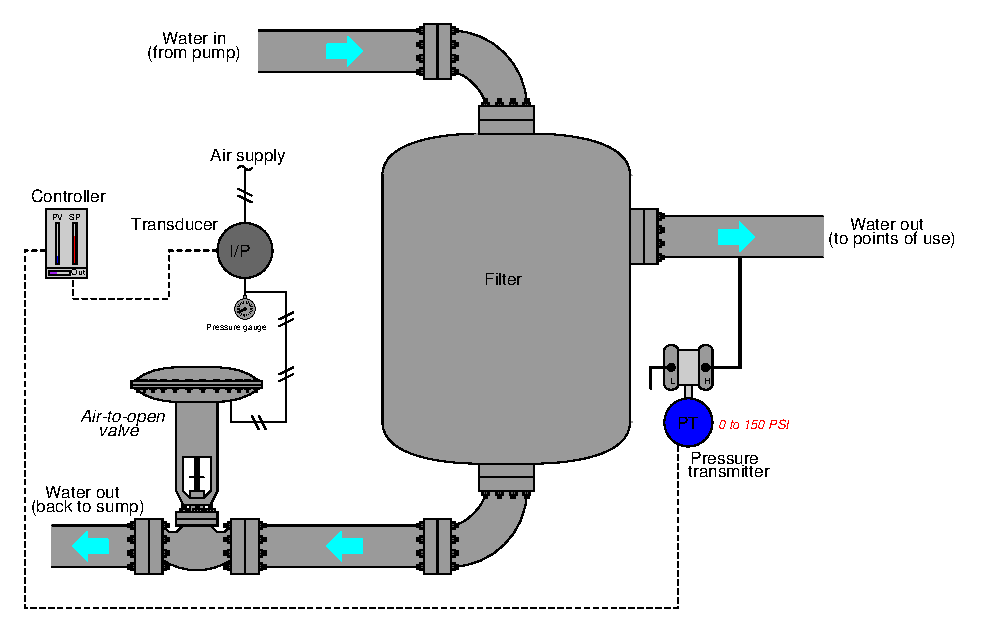
\includegraphics[width=15.5cm]{i00338x01.eps}$$

Første test er å måle sløyfestrøm i kretsen mellom trykktransmitter og trykkregulator. Multimeteret viser 6.88 mA. Neste steg er å lese av trykkmåleren (på I/P-utgangsrøret): 7.5 PSI.

\vskip 10pt

Vurder sannsynligheten for hver oppgitt feil i dette reguleringssystemet. Se på én feil om gangen (altså ingen sammenfallende feil), og avgjør om hver feil alene kan forklare \textit{alle} målinger og symptomer i kretsen.

% No blank lines allowed between lines of an \halign structure!
% I use comments (%) instead, so that TeX doesn't choke.

$$\vbox{\offinterlineskip
\halign{\strut
\vrule \quad\hfil # \ \hfil & 
\vrule \quad\hfil # \ \hfil & 
\vrule \quad\hfil # \ \hfil \vrule \cr
\noalign{\hrule}
%
% First row
{\bf Feil} & {\bf Mulig} & {\bf Umulig} \cr
%
\noalign{\hrule}
%
% Another row
PT ute av kalibrering (sender feil strøm) &  &  \cr
%
\noalign{\hrule}
%
% Another row
PIC-inngang ute av kalibrering (tolker PV-signal feil) &  &  \cr
%
\noalign{\hrule}
%
% Another row
PIC-utgang ute av kalibrering (sender feil mA-signal til I/P) &  &  \cr
%
\noalign{\hrule}
%
% Another row
Trykkmåler ute av kalibrering (viser feil trykk) &  &  \cr
%
\noalign{\hrule}
%
% Another row
I/P ute av kalibrering (gir feil trykk ut) &  &  \cr
%
\noalign{\hrule}
%
% Another row
Reguleringsventilen er overdimensjonert &  &  \cr
%
\noalign{\hrule}
%
% Another row
Reguleringsventilen er underdimensjonert &  &  \cr
%
\noalign{\hrule}
%
% Another row
PIC er dårlig trimmet (tar dårlige reguleringsbeslutninger) &  &  \cr
%
\noalign{\hrule}
%
% Another row
Instrumentluftforsyningen har ikke fullt trykk &  &  \cr
%
\noalign{\hrule}
} % End of \halign 
}$$ % End of \vbox

\underbar{file i00338}
%(END_QUESTION)





%(BEGIN_ANSWER)

Dette er en vurdert oppgave, så det gis ikke fasit eller hint.

%(END_ANSWER)





%(BEGIN_NOTES)

Et godt diagnoseprinsipp her er \textit{korrespondanse}: sjekk hvilke variabler som samsvarer med hverandre, og hvilke som ikke gjør det. Setpunktet 110 PSI lagt inn i regulatoren er tydelig langt unna PV-verdien regulatoren viser (27 PSI).

Hvis vi tar den målte strømsignalen (6.88 mA) og omregner til tilsvarende trykk med transmitterens område 0 til 150 PSI, kan vi sammenligne beregnet trykk med regulatorvisningen. Her tilsvarer 6.88 mA et trykk på 27 PSI, som stemmer med regulatorens display. Da kan vi konkludere med at regulatorens inngang og display ikke er feilkilden, fordi regulatoren mottar et signal som tilsvarer 27 PSI og viser nettopp det.

Deretter kan vi sjekke om I/P-konverterens utgangssignal på 7.5 PSI stemmer med regulatorens utgangsvisning på 38\%. Det gjør det (38\% = 7.56 PSI i området 3--15 PSI). Dermed ser kjeden fra regulatorutgang via I/P-konverter til trykkmåler ut til å fungere.

Det sentrale spørsmålet er da hvorfor regulatoren ikke forsøker sterkere å øke trykket opp mot setpunkt, siden utgangen står på 38\% (langt fra helt stengt avløpsventil). Hvis regulatoren gjorde jobben sin riktig, ville vi forventet at den stengte ventilen helt i et forsøk på å øke filtertrykket. Siden den ikke gjør det, kan vi slutte at noe er galt med regulatorens trimning (eller at den står i manuell modus).


% No blank lines allowed between lines of an \halign structure!
% I use comments (%) instead, so that TeX doesn't choke.

$$\vbox{\offinterlineskip
\halign{\strut
\vrule \quad\hfil # \ \hfil & 
\vrule \quad\hfil # \ \hfil & 
\vrule \quad\hfil # \ \hfil \vrule \cr
\noalign{\hrule}
%
% First row
{\bf Feil} & {\bf Mulig} & {\bf Umulig} \cr
%
\noalign{\hrule}
%
% Another row
PT ute av kalibrering (sender feil strøm) &  & $\surd$ \cr
%
\noalign{\hrule}
%
% Another row
PIC-inngang ute av kalibrering (tolker PV-signal feil) &  & $\surd$ \cr
%
\noalign{\hrule}
%
% Another row
PIC-utgang ute av kalibrering (sender feil mA-signal til I/P) &  & $\surd$ \cr
%
\noalign{\hrule}
%
% Another row
Trykkmåler ute av kalibrering (viser feil trykk) &  & $\surd$ \cr
%
\noalign{\hrule}
%
% Another row
I/P ute av kalibrering (gir feil trykk ut) &  & $\surd$ \cr
%
\noalign{\hrule}
%
% Another row
Reguleringsventilen er overdimensjonert &  & $\surd$ \cr
%
\noalign{\hrule}
%
% Another row
Reguleringsventilen er underdimensjonert &  & $\surd$ \cr
%
\noalign{\hrule}
%
% Another row
PIC er dårlig trimmet (tar dårlige reguleringsbeslutninger) & $\surd$ &  \cr
%
\noalign{\hrule}
%
% Another row
Instrumentluftforsyningen har ikke fullt trykk &  & $\surd$ \cr
%
\noalign{\hrule}
} % End of \halign 
}$$ % End of \vbox

%INDEX% Basics, control loop troubleshooting: determining cause of control problem

%(END_NOTES)
